%!TEX root = ../thesis.tex
% ******************************* Thesis Appendix A ****************************
\chapter{Hyperbolic Trigonometry} 

\noindent We start with fixing some notations:
\begin{enumerate}
	\item $P(a,\alpha,b,c,d,e)$ denotes a pentagon with four right angles such that $a,b,c,d,e$ are side-lengths and $\alpha$ is the angle formed by sides $a$ and $b$~(Figure~\ref{fig:test1}). 
	
	\item $Q(p,\alpha,q,r,\beta,s)$ denotes a quadrilateral with two right angles such that $p,q,r,s$ are side-lengths and $\alpha, \beta$ are the angles formed by sides $p,q$ and $r,s$ respectively~(Figure~\ref{fig:test2}). 
	
	\item A quadrilateral of the form $Q(p, \alpha,q,r,\frac{\pi}{2},s)$ is called a trirectangle~(Figure~\ref{fig:test3}).
	
\end{enumerate}



\begin{figure}[h]
	\centering
	\begin{minipage}{.5\textwidth}
		\centering
		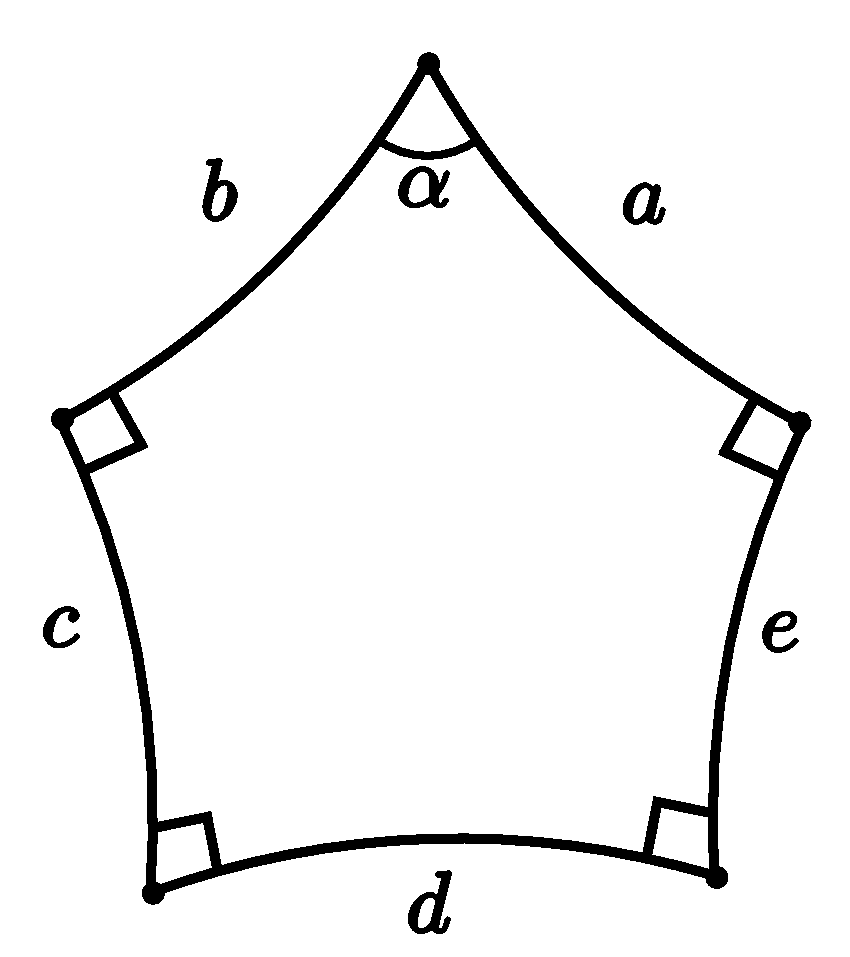
\includegraphics[width=0.7\linewidth]{Appendix1/pentagon.pdf}
		\captionof{figure}{ $P(a,\alpha,b,c,d,e)$}
		\label{fig:test1}
	\end{minipage}%
	\begin{minipage}{.5\textwidth}
		\centering
		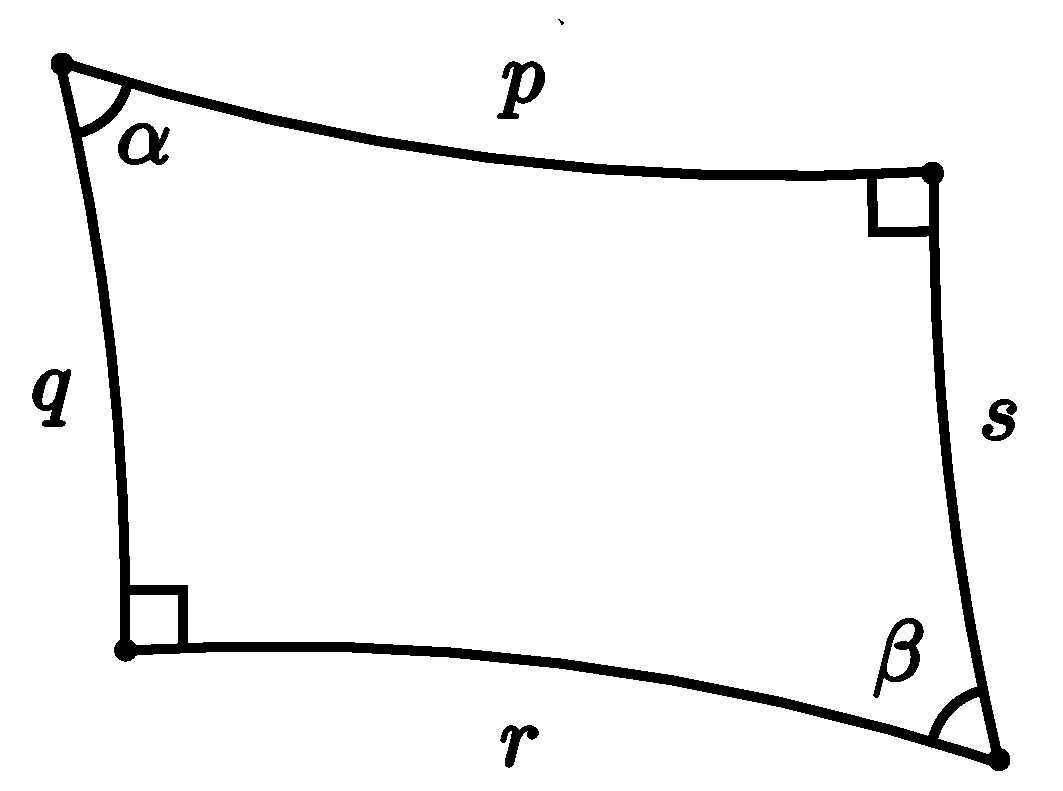
\includegraphics[width=0.7\linewidth]{Appendix1/quadrilateral.pdf}
		\captionof{figure}{ $Q(p,\alpha,q,r,\beta,s)$}
		\label{fig:test2}
	\end{minipage}
	\begin{minipage}{.5\textwidth}
		\centering
		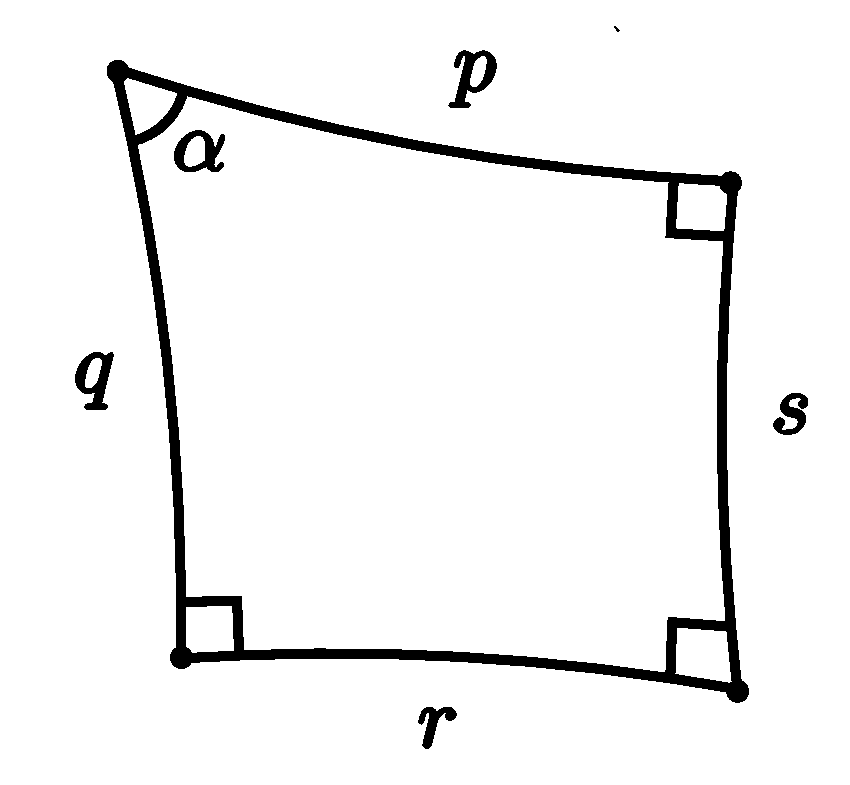
\includegraphics[width=0.7\linewidth]{Appendix1/trirectangle.pdf}
		\captionof{figure}{$Q(p, \alpha,q,r,\frac{\pi}{2},s)$}
		\label{fig:test3}
	\end{minipage}
\end{figure}

\noindent
The following theorem is taken from \cite{PB}.
\begin{theorem} {\ } 
	\label{thm:trigidentities}
	\begin{enumerate}
		\item For the pentagon $P(a,\alpha,b,c,d,e)$ we get the following identities:\vspace{0.8em}
		\begin{enumerate}
			\item $\dfrac{\cosh{a}}{\sinh{c}} = \dfrac{\cosh{b}}{\sinh{e}} =\dfrac{\sinh{d}}{\sin{\alpha}}.$\\
			\item $\cosh{d} = -\cos{\alpha} \cosh{a} \cosh{b} + \sinh{a} \sinh{b}.$ \vspace{0.8em}
			\item $\cosh{e} = -\cos{\alpha} \cosh{c} + \sin{\alpha} \sinh{b} \sinh{c}$ \vspace{0.8em}
		\end{enumerate}
		
		\item For the quadrilateral $Q(p,\alpha,q,r,\beta,s)$ we get the following identity:\vspace{0.8em}
		\begin{enumerate}
			\item $\cos{\beta} =  - \cosh{p} \cosh{q} \cos{\alpha} + \sinh{p}\sinh{q}$ \vspace{0.8em}
		\end{enumerate}
	
		\item For the trirectangle $Q(p, \alpha,q,r,\frac{\pi}{2},s)$ we get the following identities:\vspace{0.8em}
		\begin{enumerate}
			\item $\cos{\alpha} = \tanh{p} \tanh{q}$
			\vspace{0.8em}
			\item $\cos{\alpha} = \sinh{r} \sinh{s}$
		\end{enumerate}
	\end{enumerate}

	
\end{theorem}

%\begin{cor}
%	\label{cor:1}
%	Let $P(a,\alpha,b,c,d,e)$ be a pentagon, then $a = b$ iff $c = e$.
%\end{cor}
%\begin{proof}
%	This follows directly by the identity 1.($a$) in Theorem~\ref{thm:trigidentities}.
%\end{proof}
%
%\begin{cor}
%	Let $P(a,\alpha,a,c,d,c)$ be a pentagon, then $a \geq \tanh^{-1}\left({\cos{\left(\alpha/2\right)}}\right)$.
%\end{cor}
%\begin{proof}
%	It follows from the identity 1.($b$) in Theorem~\ref{thm:trigidentities} that 
%	\begin{alignat*}{2}
%		&&\sinh^2{a} - \cosh^2{a} \cos{\alpha} &= \cosh{d} \\
%		&\implies &\sinh^2{a} - \cosh^2{a} \cos{\alpha} &\geq 1 \\
%		&\implies &\tanh^2{a} - \cos{\alpha} &\geq \sech^2{a} \\
%		&\implies &2\tanh^2{a}  &\geq 1 + \cos{\alpha} \\
%		&\implies &\tanh{a} &\geq \cos{\alpha/2} \\
%		&\implies  &a &\geq \tanh^{-1}\left({\cos{\left(\alpha/2\right)}}\right)
%	\end{alignat*}
%\end{proof}
%
%\begin{cor}
%	\label{cor:2}
%	Let $Q(p,\alpha,p,r,\beta,s)$ be a quadrilateral, then $p \leq \tanh^{-1}\left({\cos{\left(\alpha/2\right)}}\right)$.
%\end{cor}
%\begin{proof}
%	It follows from the identity 2.($a$) in Theorem~\ref{thm:trigidentities} that 
%	\begin{alignat*}{2}
%		&&\sinh^2{p} - \cosh^2{p} \cos{\alpha} &= \cos{\beta} \\
%		&\implies &\sinh^2{p} - \cosh^2{p} \cos{\alpha} &\leq 1 \\
%	\end{alignat*}
%	
%	The rest follows from the proof of previous corollary.
%\end{proof}
%
%\begin{cor}
%	Let $P(a,\alpha,a,c,d,c)$ be a pentagon, then $\coth{c} = \left(\tan{\left(\alpha/2\right)}\right) \sinh{a}$.
%\end{cor}
%\begin{proof}
%	It follows from the identity 1.($c$) in Theorem~\ref{thm:trigidentities} that
%	\begin{alignat*}{2}
%		&&\cosh{c} &= -\cos{\alpha} \cosh{c} + \sin{\alpha} \sinh{a} \sinh{c} \\
%		&\implies & (1 + \cos{\alpha})\cosh{c} &= \sin{\alpha} \sinh{a} \sinh{c}\\
%		&\implies &\coth{c} &= \left(\dfrac{\sin{\alpha}}{1+\cos{\alpha}}\right) \sinh{a} \\
%		&\implies &\coth{c}  &= \left(\tan{\left(\alpha/2\right)}\right) \sinh{a} \\
%	\end{alignat*}
%\end{proof}
%
%\begin{theorem}
%	\label{thm:5}
%	For any $a > \tanh^{-1}\left({\cos{\left(\alpha/2\right)}}\right)$, there exists a unique pentagon $P(a,\alpha,a,c,d,c)$ upto isometry where $c, d$ are completely determined by $a$ and $\alpha$.
%\end{theorem}
%
%\begin{proof}
%	Consider two geodesics say $l, m$ which intersect and form an angle $\alpha$ at the origin of the Poincar\'{e} disk. Choose one point each on $l$ and $m$ such that:
%	\begin{enumerate}
%		\item they are at distance $a$ from the origin.
%		\item the geodesic arcs joining origin to these points also form an angle $\alpha$.
%	\end{enumerate}
%	\noindent
%	Draw unique perpendiculars to $l,m$ passing through these points. These perpendiculars do not intersect by Corollary~\ref{cor:2}. Now, draw the unique perpendicular of these ultra-parallel geodesics. Thus we get a pentagon of the form $P(a, \alpha, a, c, d, e)$. From Theorem~\ref{thm:trigidentities} and Corollary~\ref{cor:1}, it is clear that $c = e$ and $c, d$ are completely determined by $a, \alpha$.
%	
%	As, two  geodesics which intersect and form an angle $\alpha$ are unique upto isometry, the theorem follows. 
%\end{proof}

\begin{prop}[$\frac{1}{4}$-collars]
	\label{prop:quartercollar}
	Let $P(a,\alpha,b,c,d,e)$ be a pentagon as above.
	
	$$C_1 = \left\{z \in P ~ | ~ d(c,z) \leq \textup{arcsinh}\left(\frac{\cos\left(\alpha \right)}{\sinh{c}}\right) \right\}$$
	$$C_2 = \left\{z \in P ~ | ~ d(e,z) \leq \textup{arcsinh}\left(\frac{\cos\left(\alpha \right)}{\sinh{e}}\right) \right\}$$
	Then, $C_1 \cap C_2 = \emptyset$.
\end{prop}

\begin{proof}
	
	Let $r$ be the unique perpendicular from the vertex at $\alpha$ to $d$. $r$ divides $P$ into two trirectangles $Q_1 =  Q(r,\alpha_1, b,c,\frac{\pi}{2},d_1)$ and $ Q_2 = Q(r,\alpha_2, a,e,\frac{\pi}{2},d_2)$. See Figure~\ref{fig:pent}.
	
	\begin{figure}[h] 
%		\labellist
%		\Large
%		\pinlabel $a$ at 320 350
%		\pinlabel $b$ at 100 350
%		\pinlabel $c$ at 40 150
%		\pinlabel $d_1$ at 150 20
%		\pinlabel $d_2$ at 290 20
%		\pinlabel $e$ at 380 150
%		\pinlabel $r$ at 240 180
%		\pinlabel $\alpha_1$ at 180 340
%		\pinlabel $\alpha_2$ at 240 340
%		\endlabellist
		\centering
		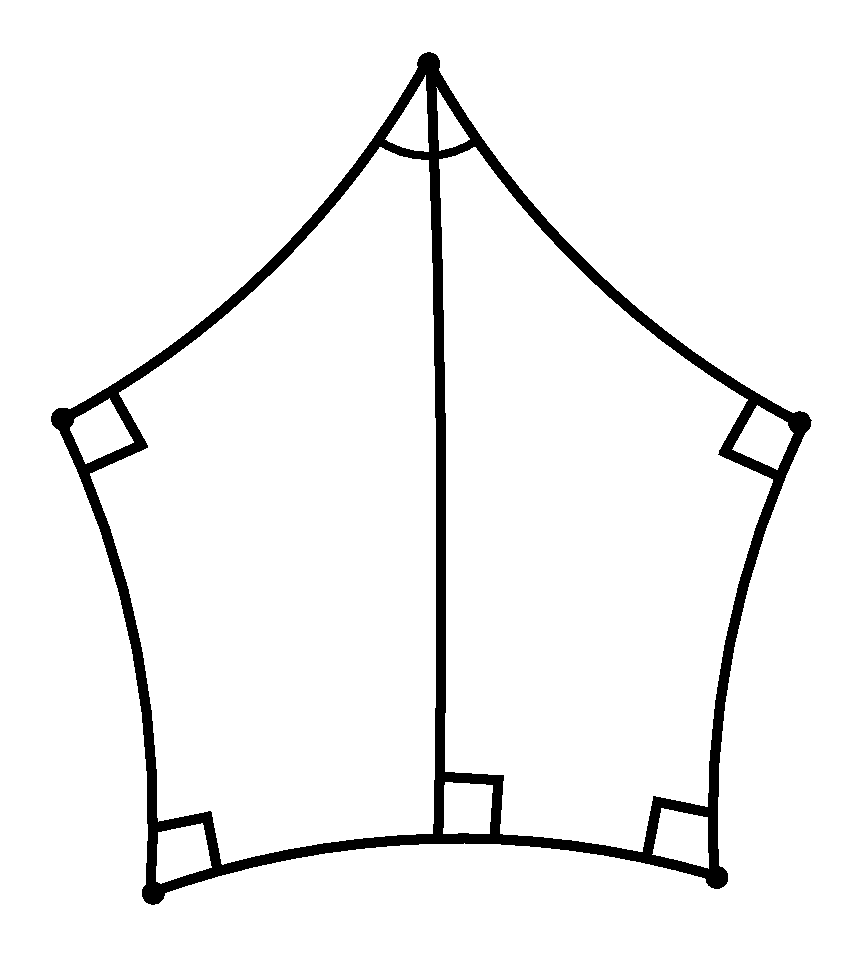
\includegraphics[width=0.3\linewidth]{Appendix1/quartercollar.pdf}
		\caption{1/4- Collars}
		\label{fig:pent}
	\end{figure}
	
	\noindent
	From 3.($b$) of Theorem~\ref{thm:trigidentities}, we get that
	$$ \sinh{c} \cdot \sinh{d_1} =  \cos{\left(\frac{\alpha_1}{2}\right)} \implies d_1 = \textup{arcsinh}\left(\frac{\cos\left(\frac{\alpha_1}{2} \right)}{\sinh{c}}\right) \leq \textup{arcsinh}\left(\frac{\cos{\alpha} }{\sinh{c}}\right)$$
	$$ \sinh{e} \cdot \sinh{d_2} =  \cos{\left(\frac{\alpha_2}{2}\right)} \implies d_2 = \textup{arcsinh}\left(\frac{\cos\left(\frac{\alpha_2}{2} \right)}{\sinh{e}}\right) \leq \textup{arcsinh}\left(\frac{\cos{\alpha}}{\sinh{e}}\right)$$
	The inequality follows because arcsinh is an increasing function. The statement follows. 
\end{proof}



Given two pentagons $P_1 \coloneqq P(a_1,\frac{\alpha}{2},b_1,c_1,d_1,e_1)$ and $ P_2 \coloneqq P(a_1,\frac{\alpha}{2},b_1,c_2,d_1,e_2)$, we can construct a $V$-piece as follows: Identify $P_1$ and $P_2$ via the sides of lengths $a_1, b_1, d_1$ to get a $V$-piece with coneangle $\alpha$. The following theorem proves that every $V$-piece is obtained by such a construction.

\begin{theorem}
	\label{thm:8}
	Let $H$ be a $V$-piece with cone angle $\alpha < 2 \pi$ and $\delta_1, \delta_2$ be the boundary geodesics of $H$. Then, there exists a pentagon $P(a,\frac{\alpha}{2},b,\frac{l(\delta_1)}{2},d,\frac{l(\delta_2)}{2})$ such that $H$ is obtained by the construction above using two copies of $P$. In other words, a $V$-piece is completely determined upto isometry by the triple $(\alpha, \delta_1,\delta_2)$. 
\end{theorem}
\begin{proof}
	Consider a $V$-piece with cone angle $\alpha < 2\pi$ and let $p$ denote the cone point. Then, there exists minimal length geodesics $a_1,a_2$ joining $p$ to boundary geodesics $\delta_1, \delta_2$ respectively and a minimal length geodesic $a_3$ between $\delta_1, \delta_2$. Moreover, $a_1,a_2,a_3$ intersect these boundary geodesics perpendicularly.
	
	Cutting the cylinder along these geodesics, we get two pentagons $P_1 = P(a,\alpha_1,b,c_1,d,c_2)$ and $P_2 = P(a,\alpha_2,b,c_1^\prime,d,c_2^\prime)$, where $c_1+ c_1^\prime = l(\delta_1), c_2  + c_2^\prime = l(\delta_2) , \alpha_1 + \alpha_2 = \alpha$. By Theorem~\ref{thm:trigidentities}, $P_1$ is isometric to $P_2$. Therefore, $c_1 = c_1^\prime = \frac{l(\delta_1)}{2}, c_2 = c_2^\prime = \frac{l(\delta_2)}{2}$ and $\alpha_1 = \alpha_2 = \frac{\alpha}{2}$.
\end{proof}

\begin{lem}[Collar Lemma for $V$-Pieces]
	\label{lem:collarlemmaV}
	Let $\delta_ 1$ an $\delta_2$ be the two closed boundary geodesics of $V$-piece $H$ with coneangle $\alpha$ . Define
	$$\mathcal{C}(\delta_i)=\left\{z \in H ~ | ~ d(\delta_i,z) \leq \textup{arcsinh}\left(\frac{\cos\left(\frac{\alpha}{2} \right)}{\sinh{\frac{l(\delta_i)}{2}}}\right) \right\}, \textup{for } i = 1, 2.$$
	
	Then, $\mathcal{C}(\delta_i)$'s are disjoint and isometric to hyperbolic cylinders.
\end{lem}
\begin{proof}
	By Theorem~\ref{thm:8}, we obtain a pentagon $P = P(a,\frac{\alpha}{2},b,\frac{l(\delta_1)}{2},d,\frac{l(\delta_2)}{2})$. Then, Proposition~\ref{prop:quartercollar} gives us the Collar Lemma.
\end{proof}

\begin{lem}[Collar Lemma for $Y$-Pieces]\cite[Proposition 3.1.8]{BM}
	\label{lem:collarlemmaY} Let $\sigma_1, \sigma_2$ and $\sigma_3$ be the three boundary geodesics of a $Y$-piece $P$. Define
		$$\mathcal{C}(\sigma_i)=\left\{z \in P ~\vert~ d(\sigma_i, z) \leq \textup{arcsinh}\left(\frac{1}{\sinh{\frac{l(\sigma_i)}{2} }}\right)\right\} \textup{for } i= 1,2,3.$$	
		Then, $\mathcal{C}(\sigma_i)$'s are pairwise disjoint and isometric to hyperbolic cylinders.
\end{lem}
